\begin{frame}
\frametitle{Виртуализация памяти}
\begin{itemize}
  \item<1-> \emph{VMM} должен разделить физическую память между \emph{VM}
    \begin{itemize}
      \item так чтобы у каждая ОС считала, что имеет дело с физической памятью;
      \item используя \emph{paging} мы можем делать с памятью все, что захотим;
      \item но современные ОС сами используют \emph{paging};
    \end{itemize}
  \item<2-> Мы можем перехватывать подмену корня таблицы страниц:
    \begin{itemize}
      \item обычно это привилигированная инструкция, например, запись в
            \emph{\%cr3} в x86;
      \item как отслеживать измения на других уровнях? (вы уже можете сами
            догадаться, как это сделать)
    \end{itemize}
\end{itemize}
\end{frame}

\begin{frame}
\frametitle{Адресные пространства}
\begin{itemize}
  \item<1-> Раньше у нас было два адресных пространства:
    \begin{itemize}
      \item \emph{Virtual Address Space} - адресное пространство, которое
            создает ОС для себя и процессов;
      \item \emph{Physical Address Space} - физическая память;
    \end{itemize}
  \item<2-> С повялением \emph{VMM} ситуация меняется:
    \begin{itemize}
      \item \emph{Virtual Address Space (VA)} - адресное пространство, которое
            создает ОС;
      \item \emph{Physical Address Space (PA)} - то, что ОС считает физической
            памятью;
      \item \emph{Machine Address Space (MA)} - настоящая физическая память;
    \end{itemize}
\end{itemize}
\end{frame}

\begin{frame}
\frametitle{Адресные пространства}
\begin{itemize}
  \item<1-> Теперь нам нужно поддержвать два отображения:
    \begin{itemize}
      \item оборудование поддерживает аппаратно только одно отображение;
      \item как эффективно поддержать оба?
    \end{itemize}
  \item<2-> Мы можем отслеживать два типа изменений отображения \emph{VA} на
        \emph{PA}:
    \begin{itemize}
      \item изменение корня таблицы страниц;
      \item изменение записи в одной из таблиц отображения;
    \end{itemize}
\end{itemize}
\end{frame}

\begin{frame}
\frametitle{Shadow Tables}
\begin{itemize}
  \item<1-> ОС подменяет корень отображения
    \begin{itemize}
      \item \emph{VMM} знает отображение \emph{PA} на \emph{MA};
      \item \emph{VMM} знает корень отображения и может пройтись по всему
            дереву таблиц страниц;
      \item \emph{VMM} просто создает новое отображение \emph{VA} напрямую на
            \emph{MA};
    \end{itemize}
  \item<2-> ОС подменяет запись в таблице
    \begin{itemize}
      \item в этом случае просто обновляем созданное отображение;
    \end{itemize}
\end{itemize}
\end{frame}

\begin{frame}
\frametitle{Пример}
\only<1>{\begin{figure}
  \centering\includegraphics[width=.8\linewidth]{shadow1}
  \caption{Shadow Page Table}
\end{figure}}
\only<2>{\begin{figure}
  \centering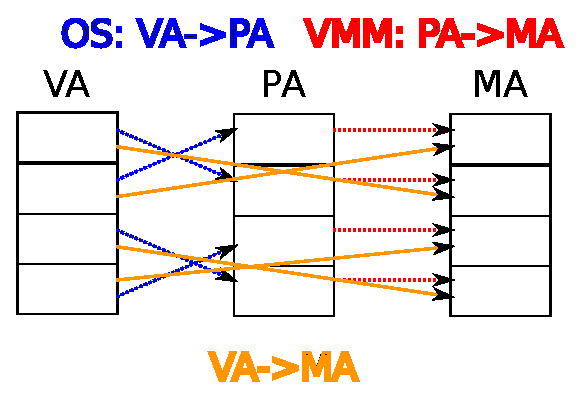
\includegraphics[width=.8\linewidth]{shadow2}
  \caption{Shadow Page Table}
\end{figure}}
\end{frame}

\begin{frame}
\frametitle{Аппаратная поддержка}
\begin{itemize}
  \item В процессоры x86 были добавлены расширения \emph{EPT} и \emph{RVI},
        которые добавляют аппаратную поддержку трансляции памяти
    \begin{itemize}
      \item как обычно, обе технологии делают одно и тоже, разница в деталях;
      \item фактически они позволяют гиппервизору задать отображение \emph{PA}
            на \emph{MA}, так чтобы ОС ничего о нем не знала;
      \item отображение \emph{PA} на \emph{MA} меняется редко, поэтому
            \emph{VMM} почти не приходится вмешиваться;
    \end{itemize}
\end{itemize}
\end{frame}

\begin{frame}
\frametitle{Balloon (bonus)}
\begin{itemize}
  \item<1-> Перераспределение памяти в ОС:
    \begin{itemize}
      \item в ОС, если вы хотите освободить память вы делаете \emph{swapping};
      \item т. е. сохраняете содержимое страниц на диске, и отдаете страницы
            памяти кому-то другому;
    \end{itemize}
  \item<2-> Перераспределение памяти в \emph{VMM}:
    \begin{itemize}
      \item \emph{VMM} запускает несколько экземпляров ОС, которые умеют делать
            сложный \emph{swapping};
      \item напишем для ОС драйвер, который знает о существовании \emph{VMM},
            назовем его \emph{balloon};
      \item если \emph{VMM} хочет забрать часть памяти у ОС, просим
            \emph{balloon} выделить нужное количество памяти (надуваем
            \emph{balloon});
      \item если \emph{VMM} решает вернуть память, просто просим драйвер
            освободить память (сдуваем \emph{balloon});
    \end{itemize}
\end{itemize}
\end{frame}
